% Beamer presentation for Etapa 1 - Trabalho Final (improved)
% Ready to paste into Overleaf (main.tex). Add 'logo.png' to project for branding.
\documentclass[11pt]{beamer}
\usetheme{Madrid}
\usecolortheme{dolphin}
\usefonttheme{professionalfonts}
\usepackage[utf8]{inputenc}
\usepackage[portuguese]{babel}
\usepackage{graphicx}
\usepackage{hyperref}
\usepackage{booktabs}
\usepackage{tikz}
\setbeamertemplate{navigation symbols}{}

\title[Etapa 1 -- Concepção]{TRABALHO FINAL -- ETAPA 1\\Concepção e Arquitetura Inicial}
\author{Leonardo Cardoso \\ Matrícula: 32021BSI004}
\institute{Disciplina: Sistemas Distribuídos}
\date{11 de Maio de 2026}
\logo{\includegraphics[height=8mm]{logo.png}}

\begin{document}

\begin{frame}
  \titlepage
  \vfill
  \centering\small Projeto: Painel IoT Distribuído com Monitoramento em Tempo Real
\end{frame}

\begin{frame}{Sumário}
  \tableofcontents
\end{frame}

% ------------------------- Visão Geral -------------------------
\section{Visão Geral}
\begin{frame}{Visão Geral do Projeto}
  \begin{itemize}
    \item Painel IoT distribuído para monitoramento em tempo real
    \item Coleta com ESP32, transmissão por MQTT, persistência em TimescaleDB
    \item Dashboard web para visualização e controle remoto
  \end{itemize}
  \vfill
  \footnotesize{Nota do orador: enfatizar motivação (escala, baixa latência, aprendizagem de SD).}
\end{frame}

% ------------------------- Arquitetura -------------------------
\section{Arquitetura}
\begin{frame}{Arquitetura (Resumo)}
  \begin{itemize}
    \item Sensores: ESP32 nodes (publicam MQTT)
    \item Broker: Mosquitto (pub/sub)
    \item API Gateway: Node.js (ingest HTTP)
    \item Backend: Node.js + dashboard (porta 3000)
    \item Banco: PostgreSQL/TimescaleDB (porta 5432) em Raspberry Pi
    \item Rede: Local + Tailscale (Funnel para acesso público)
  \end{itemize}
  \vfill\footnotesize{Dica: abra o diagrama UML se precisar (arquivo .puml no repositório).}
\end{frame}

\begin{frame}{Diagrama de Alto Nível}
  \centering
  % If you upload a PNG/SVG of the PlantUML diagram as 'arquitetura.png', it will display here.
  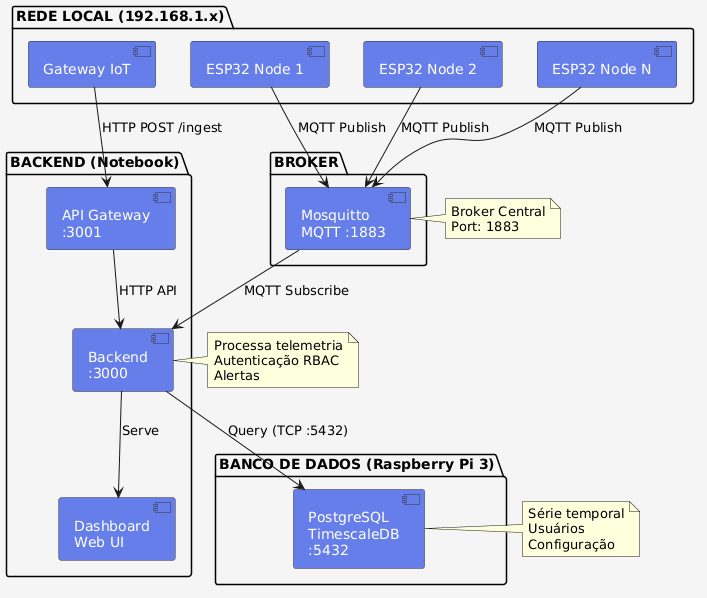
\includegraphics[width=0.9\textwidth]{arquitetura.png}
  \vfill\footnotesize{Se a imagem não estiver disponível, use o diagrama textual no apêndice do documento.}
\end{frame}

% ------------------------- Componentes -------------------------
\section{Componentes}
\begin{frame}{Componentes Principais}
  \begin{itemize}
    \item \textbf{ESP32 Nodes} -- aquisição e pré-processamento
    \item \textbf{Mosquitto} -- broker MQTT centralizado
    \item \textbf{API Gateway} -- ingest e validação
    \item \textbf{Backend} -- processamento, alertas, UI
    \item \textbf{TimescaleDB} -- armazenamento de séries temporais
  \end{itemize}
  \vfill\footnotesize{Nota do orador: preparar um exemplo de telemetria antes da demo.}
\end{frame}

\begin{frame}{ESP32 Nodes}
  \begin{itemize}
    \item Publicam tópico: `/telemetry/{device}/sensor`
    \item QoS 1, mensagens pequenas (~20-200B)
    \item Reconexão automática e buffer local
  \end{itemize}
  \vfill\footnotesize{Demonstração rápida: mostrar payload JSON de exemplo.}
\end{frame}

\begin{frame}{Broker Mosquitto}
  \begin{itemize}
    \item Papel: roteamento e retenção mínima
    \item Topologias futuras: cluster MQTT para escalabilidade
  \end{itemize}
  \vfill\footnotesize{Mencionar limites de retenção e QoS.}
\end{frame}

\begin{frame}{Backend e BD}
  \begin{itemize}
    \item Backend: Node.js processando streams e salvando em DB
    \item TimescaleDB: hypertables para telemetria (query eficiente)
  \end{itemize}
  \vfill\footnotesize{Dica técnica: use índices por dispositivo e intervalo de tempo.}
\end{frame}

% ------------------------- Fluxos e Demo -------------------------
\begin{frame}{Fluxos Principais}
  \textbf{Telemetria:} ESP32 → MQTT → Backend → TimescaleDB
  \vspace{0.3cm}
  \textbf{Comando:} Dashboard → Backend → MQTT publish → ESP32
  \vfill\footnotesize{Nota: destacar latência observada durante testes (~1-3s).}
\end{frame}

\section{Demonstração}
\begin{frame}{Demo (Passos)}
  \begin{enumerate}
    \item Verificar `tailscale status` (conectividade)
    \item Acessar dashboard: \url{https://serverl.taila7d06b.ts.net}
    \item Mostrar leitura em tempo real e enviar um comando
  \end{enumerate}
  \vfill\footnotesize{Se o Funnel estiver indisponível, usar acesso direto via IP Tailscale.}
\end{frame}

\section{Conclusão}
\begin{frame}{Conclusão e Próximos Passos}
  \begin{itemize}
    \item Projeto atende objetivos de Etapa 1 (concepção e arquitetura)
    \item Próximas etapas: concorrência, replicação, segurança avançada
    \item Agradecimentos e perguntas
  \end{itemize}
\end{frame}

% ------------------------- Apêndice / Backup -------------------------
\begin{frame}{Backup: Comandos Úteis}
  \begin{itemize}
    \item `tailscale status` -- verificar conexões
    \item `psql -h 100.82.140.119 -U iot_user -d iot_monitoring -c "SELECT count(*) FROM telemetry;"`
    \item `curl -I https://serverl.taila7d06b.ts.net` -- testar endpoint
  \end{itemize}
  \vfill\footnotesize{Tenha uma cópia offline dos slides e do PDF no pendrive antes da apresentação.}
\end{frame}

\end{document}
